
\colorlet{myblue}{blue!50}
\colorlet{orange}{orange}

\def\batchscale{0.6}
\def\batchyscale{0.45}
\def\batchcol{myblue}
\def\batchtcol{orange}

\begin{figure}[htp]
    \centering
    \begin{subfigure}[b]{0.45\textwidth}
        \centering
        \begin{tikzpicture}[label distance=-3mm]
            \clip(-1.8,-2.7) rectangle (6.1,2);
            \node[inner sep=0pt,label={below:Batch Size = 64}] (sixty) at (0,0)
                {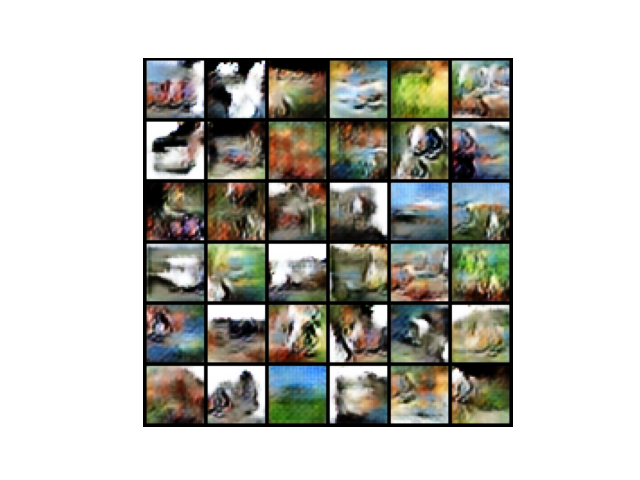
\includegraphics[scale=0.4]{Reply_to_comments_v2/images/64-30.png}};
            \node[inner sep=0pt,right = -2.4 cm of sixty,label={below:Batch Size = 16}] (sixteen)
                {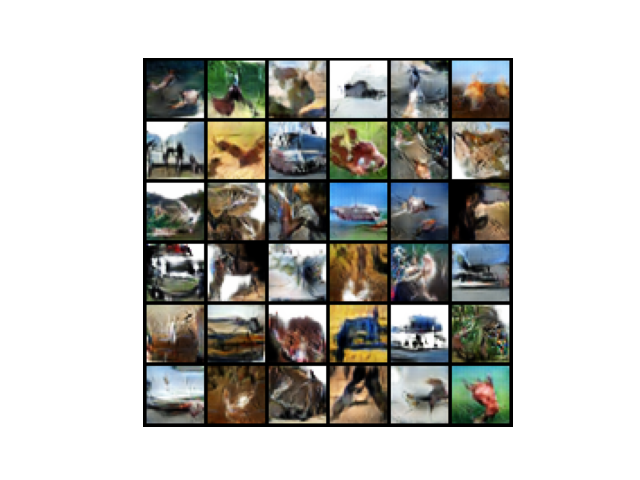
\includegraphics[scale=0.4]{Reply_to_comments_v2/images/16-30.png}};
        \end{tikzpicture}
        \caption{Output at 30 epochs}
    \end{subfigure}
    \hfill
    \begin{subfigure}[b]{0.45\textwidth}
        \centering
        \begin{tikzpicture}[scale=\batchscale]
            \begin{axis} [
                xlabel={Training Step},
                ylabel={FID Score},
                ylabel near ticks,
                ylabel shift=-10pt,
                axis x line=bottom,
                axis y line*=left,
                yticklabels={},
xtick={0,5000,10000,15000,20000,25000,30000},
xticklabels={0,5k, 10k, 15k, 20k, 25k,30k},
scaled ticks=false,
                line width=2pt
                ]
                \addplot[\batchcol, line width=2pt] table [col sep=comma,header=true,x index=0,y index=1] {Reply_to_comments_v2/batch-size-smooth.csv};
                \addplot[\batchtcol, line width=2pt] table [col sep=comma,header=true,x index=0,y index=2] {Reply_to_comments_v2/batch-size-smooth.csv};
                \legend{Batch Size 64, Batch Size 16}
            \end{axis}
        \end{tikzpicture}
        \caption{FID score comparison}
    \end{subfigure}
    \caption{The batch size effect on performance for the image-based GAN model}
    \label{fig:batch-size}
\end{figure}